So far, we focused on finding a solution that satisfies all the set of constraints, but also we have an objective function to discover the \textbf{best solution}
possible. Formally, a Constraint Optimization Problem is defined by the following sequence:
$$ \langle X, D, C, f \rangle $$
where:
\begin{itemize}
    \renewcommand{\labelitemi}{-}
    \item $X \rightarrow$ set of decision variables
    \item $D \rightarrow$ domains of the decision variables
    \item $C \rightarrow$ set of constraints between the decision variables
    \item $f \rightarrow$ formalization of the optimization criterion as an objective function
\end{itemize}
\textbf{How does the solver behave to find the best solution given a specific objective function}? \\
It uses a particular algorithm called \textbf{branch and bound algorithm}. This algorithm discovers the optimal solution (\textit{COP}) solving a sequence of
CSPs. Everytime the algorithm solves a Constraint Satisfaction Problem of the previous list, we incorporate a new constraint, named \textbf{bounding constraint},
before solving the following one. More formally, it follows three main steps:
\begin{enumerate}
    \item Each time a feasible solution is found, \textbf{posts} a new bounding constraint which ensures that a future solution must be better than it.
    \item \textbf{Backtracks} to the last decision and looks for a new solution with the additional bounding constraint, using the same search tree.
    \item \textbf{Repeats} the same process until it becomes unfeasible, the last solution found would be the optimal one.
\end{enumerate}
\begin{example}[title = Optimal map colouring]
    e.g. What is the minimum number of colors to colour a map? \vspace{3.5pt}
    \begin{center}
        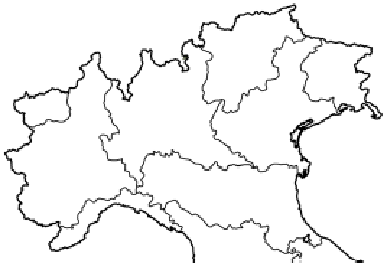
\includegraphics[width = 0.3\textwidth]{img/img4.png}
    \end{center} \vspace{3.5pt}

    \textbf{Decision variables and domains}. \\
    Every decision variable would be a region and any single domain value represents a different color. More formally, $X_i$ with $i \in \{1, \dots, n\}$ 
    are the decision variables, while \{1, \dots, n\} it's the domain. \vspace{7pt}

    \textbf{Constraints}.
    \begin{itemize}
        \renewcommand{\labelitemi}{-}
        \item $X_i \neq X_j$ for each neighboring region $i$ and $j$.
    \end{itemize} \vspace{7pt}

    \textbf{Objective function}.
    \begin{itemize}
        \renewcommand{\labelitemi}{-}
        \item $f(X) = max(X_i)$
        where:
        \begin{itemize}
            \item $X_i \rightarrow$ number of colors used
            \item $max(\dots) \rightarrow$ maximize the number of colors used
        \end{itemize}
    \end{itemize} \vspace{7pt}

    \textbf{Objective}.
    \begin{itemize}
        \renewcommand{\labelitemi}{-}
        \item $min(f(X))$
    \end{itemize}
    In order to obtain the minimum number of colors we have to minimize the objective function $f$. \vspace{3.5pt}
    \begin{center}
        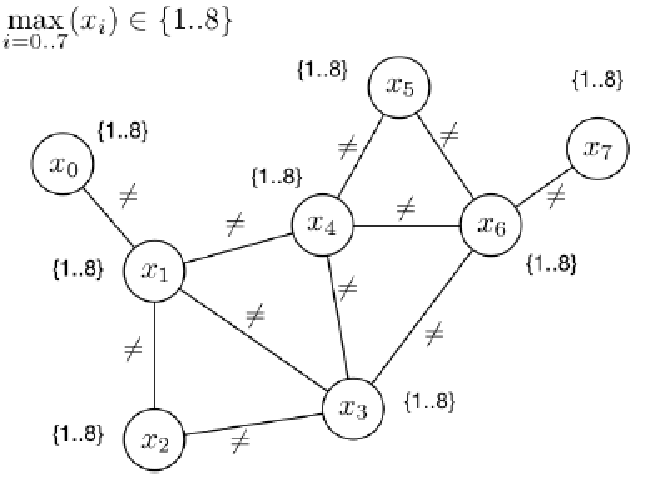
\includegraphics[width = 0.5\textwidth]{img/img20.png}
    \end{center} \vspace{3.5pt}

    The same problem can be expressed as a graph, where links between variables represent neighboring regions. What makes this problem difficult is the 
    optimality, namely find the minimum number of colors. The algorithm works as follows:
    \begin{enumerate}
        \item Pick a variable.
        \item Assign a color to the variable.
        \item Propagate the constraints involved.
    \end{enumerate} \vspace{3.5pt}
    \begin{center}
        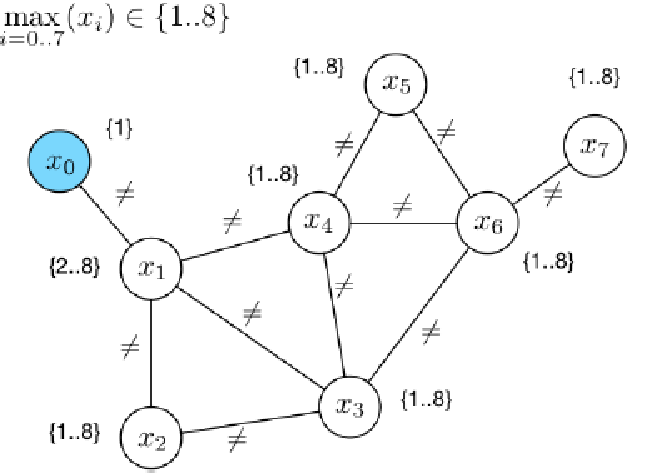
\includegraphics[width = 0.45\textwidth]{img/img21.png}
        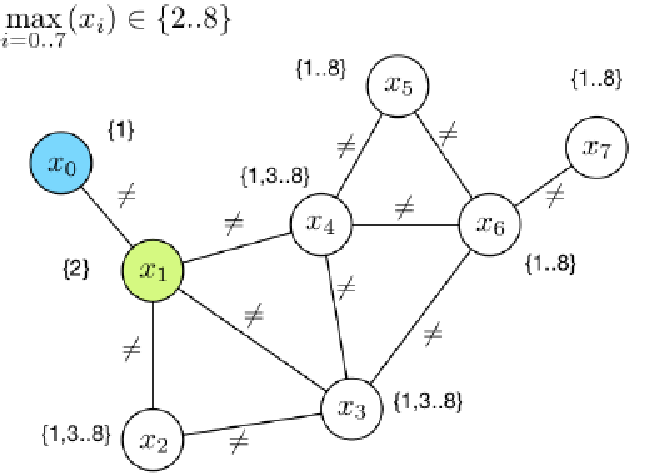
\includegraphics[width = 0.45\textwidth]{img/img22.png}
    \end{center} \vspace{3.5pt}

    We maximized the number of colors, finding a feasible solution for the first Constraint Satisfaction Problem. Now we backtrack to the last decision 
    done and we add an additional bounding constraint, $\textit{max}_{i = 0 \dots 7}(X_i) < 4$. We have a new constraint to satisfy and, as we can observe 
    from the image above, we fail: we cannot choose any value less than $4$. \vspace{3.5pt}
    \begin{center}
        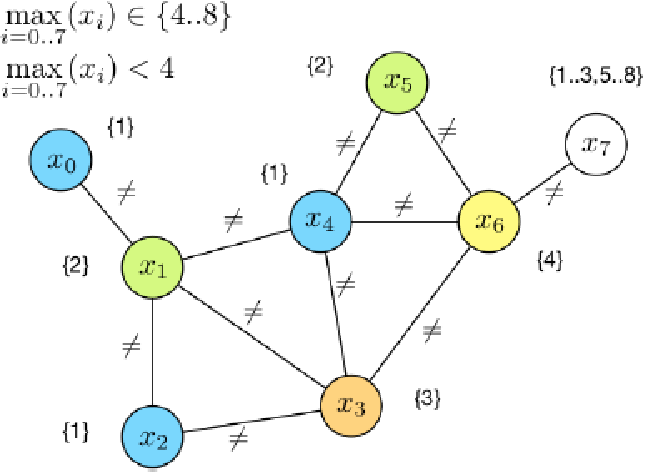
\includegraphics[width = 0.45\textwidth]{img/img23.png}
        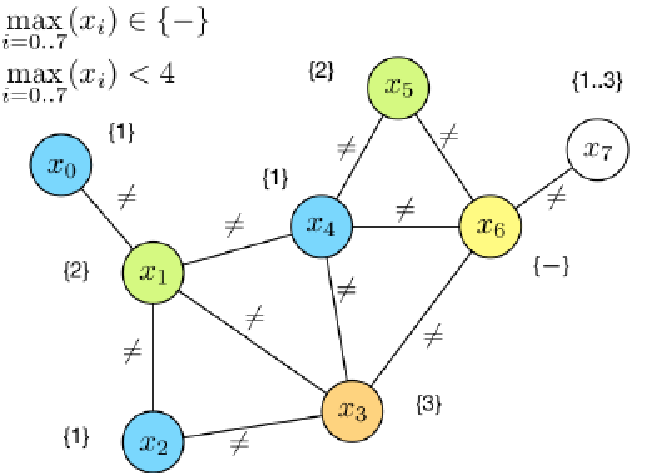
\includegraphics[width = 0.45\textwidth]{img/img24.png}
    \end{center} \vspace{3.5pt}

    Therefore, we go one level higher, doing another backtrack step, until we reach a potential feasible resolution of the problem. \vspace{3.5pt}
    \begin{center}
        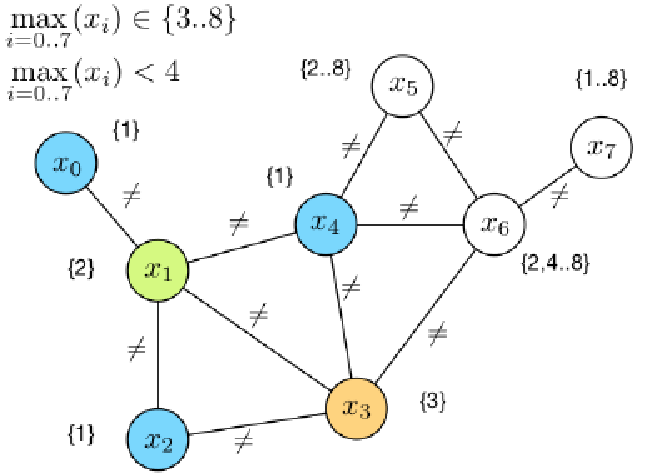
\includegraphics[width = 0.45\textwidth]{img/img25.png}
        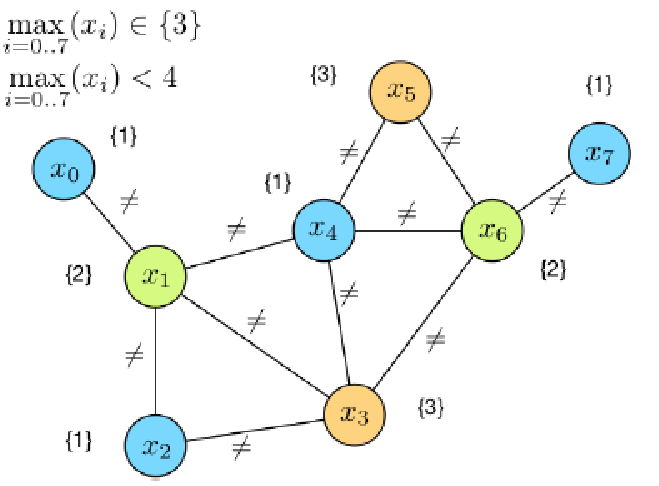
\includegraphics[width = 0.45\textwidth]{img/img26.png}
    \end{center} \vspace{3.5pt}
\end{example}